% 定理环境3

\ifx\allfiles\undefined
\documentclass[12pt, a4paper, oneside, UTF8]{ctexbook}  % +  这一句是新增加的
% \documentclass[12pt, a4paper,oneside, UTF8]{ctexbook}
% \usepackage[dvipsnames]{xcolor}   % (环境2)删除
\usepackage[dvipsnames, svgnames]{xcolor} % (环境2)替换原来的 \usepackage[dvipsnames]{xcolor}
\usepackage[strict]{changepage} % (环境2)添加
\usepackage{framed}             % (环境2)添加
\usepackage{amsmath}   % 数学公式
\usepackage{amsthm}    % 定理环境
\usepackage{amssymb}   % 更多公式符号
\usepackage{graphicx}  % 插图
\usepackage{mathrsfs}  % 数学字体
\usepackage{enumitem}  % 列表
\usepackage{geometry}  % 页面调整
\usepackage{unicode-math}
\usepackage[colorlinks,linkcolor=black]{hyperref}

\usepackage{titling}    % 封面添加的

\usepackage{tcolorbox}  % (环境1)添加的
\tcbuselibrary{most}    % (环境1)添加的

\graphicspath{ {figure/},{../figure/}, {config/}, {../config/} }  % 配置图形文件检索目录
\linespread{1.5} % 行高

% 页码设置
\geometry{top=25.4mm,bottom=25.4mm,left=20mm,right=20mm,headheight=2.17cm,headsep=4mm,footskip=12mm}

% 设置列表环境的上下间距
\setenumerate[1]{itemsep=5pt,partopsep=0pt,parsep=\parskip,topsep=5pt}
\setitemize[1]{itemsep=5pt,partopsep=0pt,parsep=\parskip,topsep=5pt}
\setdescription{itemsep=5pt,partopsep=0pt,parsep=\parskip,topsep=5pt}



% % 原始定理环境
% % ########## 定理环境 start ##############################################################
% \theoremstyle{definition}
% \newtheorem{defn}{\indent 定义}[section]

% \newtheorem{lemma}{\indent 引理}[section]    % 引理 定理 推论 准则 共用一个编号计数
% \newtheorem{thm}[lemma]{\indent 定理}
% \newtheorem{corollary}[lemma]{\indent 推论}
% \newtheorem{criterion}[lemma]{\indent 准则}

\newtheorem{proposition}{\indent 命题}[section]
\newtheorem{example}{\indent \color{SeaGreen}{例}}[section] % 绿色文字的 例 ,不需要就去除\color{SeaGreen}{}
\newtheorem*{rmk}{\indent 注}

% % 两种方式定义中文的 证明 和 解 的环境:
% % 缺点:\qedhere 命令将会失效【技术有限,暂时无法解决】
\renewenvironment{proof}{\par\textbf{证明.}\;}{\qed\par}
\newenvironment{solution}{\par{\textbf{解.}}\;}{\qed\par}

% % 缺点:\bf 是过时命令,可以用 textb f等替代,但编译会有关于字体的警告,不过不影响使用【技术有限,暂时无法解决】
% %\renewcommand{\proofname}{\indent\bf 证明}
% %\newenvironment{solution}{\begin{proof}[\indent\bf 解]}{\end{proof}}
% % ######### 定理环境 end  ##############################################################





% % #### 将 config.tex 中的定理环境的对应部分替换为如下内容   (环境2)
% % 定义单独编号,其他四个共用一个编号计数 这里只列举了五种,其他可类似定义(未定义的使用原来的也可)
% \newtcbtheorem[number within=section]{defn}%
% {定义}{colback=OliveGreen!10,colframe=Green!70,fonttitle=\bfseries}{def}

% \newtcbtheorem[number within=section]{lemma}%
% {引理}{colback=Salmon!20,colframe=Salmon!90!Black,fonttitle=\bfseries}{lem}

% % 使用另一个计数器 use counter from=lemma
% \newtcbtheorem[use counter from=lemma, number within=section]{them}%
% {定理}{colback=SeaGreen!10!CornflowerBlue!10,colframe=RoyalPurple!55!Aquamarine!100!,fonttitle=\bfseries}{them}

% \newtcbtheorem[use counter from=lemma, number within=section]{criterion}%
% {准则}{colback=green!5,colframe=green!35!black,fonttitle=\bfseries}{cri}

% \newtcbtheorem[use counter from=lemma, number within=section]{corollary}%
% {推论}{colback=Emerald!10,colframe=cyan!40!black,fonttitle=\bfseries}{cor}
% % colback=red!5,colframe=red!75!black

% % 这个颜色我不喜欢
% %\newtcbtheorem[number within=section]{proposition}%
% %{命题}{colback=red!5,colframe=red!75!black,fonttitle=\bfseries}{cor}

% % .... 命题 例 注 证明 解 使用之前的就可以(全文都是这种框框就很丑了),也可以按照上述定义 ...






% #### 将 config.tex 中的定理环境的对应部分替换为如下内容   (环境3)
\definecolor{greenshade}{rgb}{0.90,1,0.92} 		% 绿色文本框,竖线颜色设为 Green
\definecolor{redshade}{rgb}{1.00,0.88,0.88}   		% 红色文本框,竖线颜色设为 LightCoral
\definecolor{brownshade}{rgb}{0.99,0.95,0.9} 		% 莫兰迪棕色,竖线颜色设为 BurlyWood
\definecolor{lilacshade}{rgb}{0.95,0.93,0.98}    	% 淡紫色,竖线颜色设为 Plum
\definecolor{orangeshade}{rgb}{1.00,0.88,0.82} 		% 橙色,竖线颜色设为 DarkOrange
\definecolor{lightblueshade}{rgb}{0.8,0.92,1} 		% 淡蓝色,竖线颜色设为 LightSkyBlue
\theoremstyle{definition}
\newtheorem{defn1}{\indent 定义}[section]
\newtheorem{lemma1}{\indent 引理}[section]
\newtheorem{thm1}[lemma1]{\indent 定理}
\newtheorem{corollary1}[lemma1]{\indent 推论}
\newtheorem{criterion1}[lemma1]{\indent 准则}
% \newtheorem*{rmk1}{\indent 注}

\newenvironment{formal}[2][]{%
    \def\FrameCommand{%
        \hspace{1pt}%
        {\color{#1}\vrule width 2pt}%
        {\color{#2}\vrule width 4pt}%
        \colorbox{#2}%
    }%
    \MakeFramed{\advance\hsize-\width\FrameRestore}%
    \noindent\hspace{-4.55pt}%
    \begin{adjustwidth}{}{7pt}\vspace{2pt}\vspace{2pt}}{%
        \vspace{2pt}\end{adjustwidth}\endMakeFramed%
}

% 定义
\newenvironment{defn}{\begin{formal}[Green]{greenshade}\begin{defn1}}{\end{defn1}\end{formal}}
% 定理
\newenvironment{thm}{\begin{formal}[LightSkyBlue]{lightblueshade}\begin{thm1}}{\end{thm1}\end{formal}}
% 引理
\newenvironment{lemma}{\begin{formal}[Plum]{lilacshade}\begin{lemma1}}{\end{lemma1}\end{formal}}
% 推论
\newenvironment{corollary}{\begin{formal}[BurlyWood]{brownshade}\begin{corollary1}}{\end{corollary1}\end{formal}}
% 准则
\newenvironment{criterion}{\begin{formal}[DarkOrange]{orangeshade}\begin{criterion1}}{\end{criterion1}\end{formal}}
% 注
% \newenvironment{rmk}{\begin{formal}[LightCoral]{redshade}\begin{rmk1}}{\end{rmk1}\end{formal}}






% ↓↓↓↓↓↓↓↓↓↓↓↓↓↓↓↓↓ 以下是自定义的命令  ↓↓↓↓↓↓↓↓↓↓↓↓↓↓↓↓

% 用于调整表格的高度  使用 \hline\xrowht{25pt}
\newcommand{\xrowht}[2][0]{\addstackgap[.5\dimexpr#2\relax]{\vphantom{#1}}}

% 表格环境内长内容换行
\newcommand{\tabincell}[2]{\begin{tabular}{@{}#1@{}}#2\end{tabular}}

% 使用\linespread{1.5} 之后 cases 环境的行高也会改变,重新定义一个 ca 环境可以自动控制 cases 环境行高
\newenvironment{ca}[1][1]{\linespread{#1} \selectfont \begin{cases}}{\end{cases}}
% 和上面一样
\newenvironment{vx}[1][1]{\linespread{#1} \selectfont \begin{vmatrix}}{\end{vmatrix}}

\def\d{\textup{d}} % 直立体 d 用于微分符号 dx
\def\R{\mathbb{R}} % 实数域
\newcommand{\bs}[1]{\boldsymbol{#1}}    % 加粗,常用于向量
\newcommand{\ora}[1]{\overrightarrow{#1}} % 向量

% 数学 平行 符号
\newcommand{\pll}{\kern 0.56em/\kern -0.8em /\kern 0.56em}

% 用于空行\myspace{1} 表示空一行 填 2 表示空两行  
\newcommand{\myspace}[1]{\par\vspace{#1\baselineskip}}

\begin{document}
% \renewcommand*{\maketitle}{
    \begin{titlepage}
        \newgeometry{margin = 0in}
        \parindent=0pt
        % 注意这里使用了一张图片,封面使用的图片放到 config文件夹下
        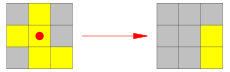
\includegraphics[width=\linewidth]{1.png}
        \vfill
        \begin{center}
            \parbox{0.618\textwidth}{
                \hfill {\bfseries \Huge \thetitle} \\[0.6pt]
                \rule{0.618\textwidth}{4pt}
            }
        \end{center}
        \vfill
        \begin{center}
            \parbox{0.618\textwidth}{
                \hfill\Large
                \begin{tabular}{r|}
                    作者:\theauthor \\
                    时间:\thedate   \\
                \end{tabular}
            }
        \end{center}
        \vfill
        \begin{center}
            \parbox[t]{0.7\textwidth}{\centering  }
        \end{center}
        \vfill
    \end{titlepage}
    \restoregeometry
    \thispagestyle{empty}
}

% 修改 名称 作者 时间
\title{自用\rm{\LaTeX}书籍模版}
\author{名字}
\date{\today}
\thispagestyle{empty}
\maketitle

\thispagestyle{empty}
\begin{center}\Huge\textbf{前言}\end{center}
前言前言前言前言前言前言前言前言前言前言前言
前言前言前言前言前言前言前言前言前言前言前言
\begin{flushright}
    \begin{tabular}{c}
        \today \\ 签名
    \end{tabular}
\end{flushright}

\newpage
\setcounter{page}{1}
\pagestyle{plain}
\pagenumbering{Roman}
\tableofcontents

\newpage
\pagestyle{plain}
\setcounter{page}{1}
\pagenumbering{arabic} % 单独编译时,其实不用编译封面目录之类的,如需要不注释这句即可
\else
\fi
%  ↓↓↓↓↓↓↓↓↓↓↓↓↓↓↓↓↓↓↓↓↓↓↓↓↓↓↓↓ 正文部分 ↓↓↓↓↓↓↓↓↓↓↓↓↓↓↓↓↓↓↓↓↓↓↓↓↓↓↓↓

\chapter{曲线积分与曲面积分}
\section{Gauss公式}

\begin{rmk}
    以下是随机选取的演示部分(仅作演示).
\end{rmk}

\begin{thm}
    设空间闭区域$\Omega$由分片光滑的闭曲面$\Sigma$围成,若函数$P(x,y,z),\;Q(x,y,z) \\ ,R(x,y,z)$在$\Omega$上具有一阶连续偏导数,则有
    \begin{equation}
        \iiint_{\Omega} \bigg(\frac{\partial P}{\partial x}+\frac{\partial Q}{\partial y}+\frac{\partial R}{\partial z} \bigg)\d v = \oiint_{\Sigma}P\d y\d z+Q\d z\d x+R\d x\d y
    \end{equation}
    或
    \begin{equation}
        \iiint_{\Omega} \bigg(\frac{\partial P}{\partial x}+\frac{\partial Q}{\partial y}+\frac{\partial R}{\partial z} \bigg)\d v = \oiint_{\Sigma}(P\cos\alpha+Q\cos\beta+R\cos\gamma)\d S
    \end{equation}
    这里$\Sigma$是$\Omega$的整个边界曲面的外侧,$\cos\alpha,\;\cos\beta,\;\cos\gamma$是$\Sigma$在点$(x,y,z)$处的法向量的单位余弦.
\end{thm}

\begin{proof}
    设闭区域$\Omega$在$xOy$平面上的投影区域为$D_{xy}$,假定穿过$\Omega$内部且平行于$z$轴的直线与$\Omega$的边界曲面$\Sigma$的交点恰是两个,可设$\Sigma$由$\Sigma_1,\;\Sigma_2$和$\Sigma_3$三部分组成,其中$\Sigma_1$和$\Sigma_2$分别由方程$z = z_1(x,y)$和$z = z_2(x,y)$给定,这里$z_1(x,y) \le z_2(x,y)$,$\Sigma_1$取下侧,$\Sigma_2$取上侧,$\Sigma_3$是以$D_{xy}$的边界曲线为准线而母线平行于$z$轴的柱面上的一部分,取外侧.

    由三重积分的计算法,有
    \begin{align*}
        \iiint_{\Omega}\frac{\partial R}{\partial z}\d v & = \iint_{D_{xy}}\bigg(\int_{z_1(x,y)}^{z_2(x,y)} \frac{\partial R}{\partial z}\d z\bigg) \d x\d y \\
                                                         & =\iint_{D_{xy}}\Big\{R\big[x,y,z_2(x,y)\big]-R\big[x,y,z_1(x,y)\big]\Big\}\d x\d y
    \end{align*}
    又由曲面积分的计算法,有
    \begin{gather*}
        \iint_{\Sigma_1}R(x,y,z)\d x\d y = -\iint_{D_{xy}}R\big[x,y,z_1(x,y) \big]\d x\d y \\
        \iint_{\Sigma_2}R(x,y,z)\d x\d y = \iint_{D_{xy}}R\big[x,y,z_2(x,y) \big]\d x\d y
    \end{gather*}
    而$\Sigma_3$上任意一块曲面在$xOy$面上的投影为零,由对坐标的曲面积分的定义可知
    \[
        \iint_{\Sigma_3}R(x,y,z)\d x\d y = 0
    \]
    上述三式相加有
    \[
        \oiint_{\Sigma}R(x,y,z)\d x\d y = \iint_{D_{xy}}\Big[R\big[x,y,z_2(x,y)\big]-R\big[x,y,z_1(x,y)\big]\Big]\d x\d y
    \]
    易得
    \[
        \iiint_{\Omega}\frac{\partial R}{\partial z}\d v = \oiint_{\Sigma}R(x,y,z)\d x\d y
    \]
    如果穿过$\Omega$内部且平行于$x$轴的直线以及平行于$y$轴的直线与$\Omega$的边界曲面$\Sigma$的的交点恰好也是两个,类似地可得
    \[
        \iiint_{\Omega}\frac{\partial P}{\partial x}\d v = \oiint_{\Sigma}P(x,y,z)\d y\d z,\enspace \iiint_{\Omega}\frac{\partial Q}{\partial y}\d v = \oiint_{\Sigma}Q(x,y,z)\d z\d x
    \]
    上述三式相加即有\textbf{Gauss}公式.
\end{proof}

\begin{example}
    求微分方程$y''-2y'-3y=3x+1$的一个特解.
\end{example}
\begin{solution}
    这是二阶常系数非齐次线性微分方程,且函数$f(x)$是$e^{\lambda{x}}P_m(x)$型,其中
    \[
        \lambda = 0,\;P_m(x) = 3x+1
    \]
    与所给方程对应的齐次方程为
    \[
        y''-2y'-3y=0
    \]
    其特征方程为
    \[
        r^2-2r-3 = 0
    \]
    由于$\lambda = 0$不是特征方程的根,所以设特解
    \[
        y* = b_0 x + b_1
    \]
    带入所给方程,得
    \[
        -3b_0 x - 2b_0 - 3b_1 = 3x+1
    \]
    比较等式两端$x$同次幂的系数,易得$b_0 = -1,\;b_1 = \dfrac{1}{3}$,于是求得一个特解为
    \[
        y* = -x + \frac{1}{3}
    \]
\end{solution}

\begin{defn}
    设二元函数$f(P) = f(x,\,y)$的定义域为$D$,点$P_0(x_0,\,y_0)$是$D$的聚点,如果存在常数$A$,对于任意给定正数$\varepsilon$,总存在正整数$\delta$,使得当点$P(x,\,y) \in D \cap \mathring{U}(P_0,\,\delta)$时,都有
    \[
        |f(P)-A| = |f(x,\,y) - A| < \varepsilon
    \]
    成立,那么就称常数$A$为函数$f(x,\,y)$当$(x,\,y) \to (x_0,\,y_0)$时的极限(二重极限),记作
    \[
        \lim_{(x,\,y) \to (x_0,\,y_0)}f(x,\,y) = A \quad \lor \quad \lim_{P \to P_0}f(P) = A
    \]
\end{defn}

\myspace{1}

任意一点$P \in \R^2$与任意一个点集$E \subset \R^2$之间有以下三种关系的一种:
\begin{itemize}[leftmargin=45pt]
    \item \textbf{内点}:如果存在点$P$的某个邻域$U(P)$,使得$U(P) \subset E$,那么称$P$为$E$的内点.
    \item \textbf{外点}:如果存在点$P$的某个邻域$U(P)$,使得$U(P) \cap E = \varnothing$,那么称$P$为$E$的外点.
    \item \textbf{边界点}:如果点$P$在任意邻域内既含有属于$E$的点,又含有不属于$E$的点,那么称$P$为$E$的边界点.
\end{itemize}


\begin{defn}[线性微分方程解的结构]
    设$y*(x)$是\textbf{二阶非齐次线性微分方程}
    \begin{equation}
        y'' + P(x)y'+Q(x)y = f(x)
    \end{equation}
    的一个特解,$Y(x)$是与(eq:7-12)对应的齐次方程(eq:7-10)的通解,则
    \begin{equation}
        y = Y(x)+y*(x)
    \end{equation}
    是二阶非齐次线性微分方程(eq:7-12)的通解.
\end{defn}

\begin{thm}[线性微分方程解的结构]
    设$y*(x)$是\textbf{二阶非齐次线性微分方程}
    \begin{equation}
        y'' + P(x)y'+Q(x)y = f(x)
    \end{equation}
    的一个特解,$Y(x)$是与(eq:7-12)对应的齐次方程(eq:7-10)的通解,则
    \begin{equation}
        y = Y(x)+y*(x)
    \end{equation}
    是二阶非齐次线性微分方程(eq:7-12)的通解.
\end{thm}

\begin{lemma}[线性微分方程解的结构]
    设$y*(x)$是\textbf{二阶非齐次线性微分方程}
    \begin{equation}
        y'' + P(x)y'+Q(x)y = f(x)
    \end{equation}
    的一个特解,$Y(x)$是与(eq:7-12)对应的齐次方程(eq:7-10)的通解,则
    \begin{equation}
        y = Y(x)+y*(x)
    \end{equation}
    是二阶非齐次线性微分方程(eq:7-12)的通解.
\end{lemma}

\begin{corollary}[线性微分方程解的结构]
    设$y*(x)$是\textbf{二阶非齐次线性微分方程}
    \begin{equation}
        y'' + P(x)y'+Q(x)y = f(x)
    \end{equation}
    的一个特解,$Y(x)$是与(eq:7-12)对应的齐次方程(eq:7-10)的通解,则
    \begin{equation}
        y = Y(x)+y*(x)
    \end{equation}
    是二阶非齐次线性微分方程(eq:7-12)的通解.
\end{corollary}

\begin{criterion}[线性微分方程解的结构]
    设$y*(x)$是\textbf{二阶非齐次线性微分方程}
    \begin{equation}
        y'' + P(x)y'+Q(x)y = f(x)
    \end{equation}
    的一个特解,$Y(x)$是与(eq:7-12)对应的齐次方程(eq:7-10)的通解,则
    \begin{equation}
        y = Y(x)+y*(x)
    \end{equation}
    是二阶非齐次线性微分方程(eq:7-12)的通解.
\end{criterion}

\begin{rmk}[线性微分方程解的结构]
    设$y*(x)$是\textbf{二阶非齐次线性微分方程}
    \begin{equation}
        y'' + P(x)y'+Q(x)y = f(x)
    \end{equation}
    的一个特解,$Y(x)$是与(eq:7-12)对应的齐次方程(eq:7-10)的通解,则
    \begin{equation}
        y = Y(x)+y*(x)
    \end{equation}
    是二阶非齐次线性微分方程(eq:7-12)的通解.
\end{rmk}

图片

\begin{figure}[htbp]
    \centering
    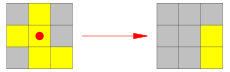
\includegraphics[scale=0.6]{1.png}
    \caption{这里是图片的说明文字}
\end{figure}

%  ↑↑↑↑↑↑↑↑↑↑↑↑↑↑↑↑↑↑↑↑↑↑↑↑↑↑↑↑ 正文部分 ↑↑↑↑↑↑↑↑↑↑↑↑↑↑↑↑↑↑↑↑↑↑↑↑↑↑↑↑
\ifx\allfiles\undefined
\end{document}
\fi